%%% LearnPAd Document template / example using learnpad.cls class for styling
%%% 20140704, 
%%% Guglielmo De Angelis <guglielmo.deangelis@isti.cnr.it>
%%% Andrea Polini <andrea.polini@unicam.it>

\documentclass{learnpad}
\usepackage[utf8]{inputenc}
\usepackage[T1]{fontenc}
\usepackage{verbatim}
\usepackage[english]{isodate}

%%% ------------------------------------------------------
%%% ---------------- The Title
%%% ------------------------------------------------------
\title{Technology-oriented Learn PAd whitepaper}

%%% ------------------------------------------------------
%%% ---------------- The Sub-Title
%%% ------------------------------------------------------
\subtitle{First version}

%%% ------------------------------------------------------
%%% ---------------- The Name of the Deliverable
%%% ------------------------------------------------------
\deliverableno{D9.5}

%%% ------------------------------------------------------
%%% ---------------- The Authors
%%% ------------------------------------------------------
\authors{
Jean Simard (XWIKI)
}

%%% ------------------------------------------------------
%%% ---------------- The Editors
%%% ------------------------------------------------------
\editors{Jean Simard}

%%% ------------------------------------------------------
%%% ---------------- The reviewers
%%% ------------------------------------------------------
\reviewers{Andrea Polini (UNICAM)}

%%% ------------------------------------------------------
%%% ---------------- The date
%%% ------------------------------------------------------
\date{\today}

%%% ------------------------------------------------------
%%% ---------------- deliverable info
%%% ---------------- choose among : Report / Other / Prototype
%%% ------------------------------------------------------
\naturedeliverable{Report}%
%%% ------------------------------------------------------
%%% ---------------- deliverable dissemination levele
%%% ---------------- choose among the two options below:
\disseminationlevelpublic
% \disseminationlevelconfidential
%%% ------------------------------------------------------
\version{2.0}%
\contractualdeliverydate{24 January 2016}%
\actualdeliverydate{24 January 2016}%
\contributingwp{WP9}%

%%% ------------------------------------------------------
%%% ---------------- abstract
%%% ------------------------------------------------------

\abstract{Provides a technology oriented overview of Learn PAd that is targeted
to readers from research and software vendor communities with a goal to build
interest in adopting Learn PAd concepts in further research and integrating
technological components in external e-learning, modelling and middleware
software applications.}

%%% ------------------------------------------------------
%%% ---------------- Keywords
%%% ------------------------------------------------------
\keywords{platform, white paper}

%%% ------------------------------------------------------
%%% ---------------- review table
%%% ------------------------------------------------------
\reviewoutline{2 Dec. 2015}{0.2}{}{}
\reviewdraft{27 Dec. 2015}{1.2}{}{}
\reviewinternal{10 Jan. 2016}{2.0}{Andrea Polini, Antonia Bertolino}{}
\reviewcandidatefinal{24 Jan. 2016}{3.0}{Antonia Bertolino}{}

\begin{document}

\frontmatter
\maketitle

%% ------------------------------------------------------
%% ---------------- document history
%% ------------------------------------------------------
\begin{history}
  \historyitem{0.1}{ToC}{Jean Simard}
  \historyitem{0.2}{ToC}{Jean Simard}
  \historyitem{1.0}{Write the Introduction}{Jean Simard}
  \historyitem{1.1}{Add Flow view and Component View}{Jean Simard}
  \historyitem{1.2}{Remove sections}{Jean Simard}
  \historyitem{2.0}{Improve after a review from XWiki}{Jean Simard}
\end{history}

%%% ------------------------------------------------------
%%% ---------------- review table with the previous info
%%% ------------------------------------------------------
\reviewtable

% %%% ------------------------------------------------------
% %%% ---------------- acronyms
% %%% ------------------------------------------------------
% \begin{acronyms}
%   \acronym{CA}{Consortium Agreement}%
%   \acronym{DL}{Deliverable Leader}%
%   \acronym{DOW}{Description of Work}%
%   \acronym{EC}{European Commission}%
%   \acronym{EL}{Exploitation Leader}%
%   \acronym{GA}{Grant Agreement}%
%   \acronym{IPR}{Intellectual Property Rights}%
%   \acronym{PAB}{Project Advisory Board}%
%   \acronym{PCB}{Project Coordination Board}%
%   \acronym{PL}{Project Leader}%
%   \acronym{PMB}{Project Management Board}%
%   \acronym{PO}{Project Officer}%
%   \acronym{SL}{Scientific Leader}%
%   \acronym{S\&T}{Scientific and Technical}%
%   \acronym{TL}{Technical Leader}%
%   \acronym{WP}{Work Package}%
%   \acronym{WPL}{Work Package Leader}
% %   \acronym{\dots}{\dots~\dots}%
% \end{acronyms}

\tableofcontents

%%% ------------------------------------------------------
% In case you don't need one of the following list 
% just comment the line
%%% ------------------------------------------------------

% \listoftables 
% \listoffigures 
% \listoflistings

%%% ------------------------------------------------------

\mainmatter

%%% ------------------------------------------------------
%%% ---------------- Start with chapter and sections here!
%%% ------------------------------------------------------

\chapter{E-Learning and Knowledge Management of processes in Public Administration}
\label{ch:intro}

\section{Why \learnpad?}
In modern society public administrations (PAs) are undergoing a transformation
of their perceived role from controllers to proactive service providers, and are
under pressure to constantly improve their service quality while coping with
quickly changing context (changes in law and regulations, societal
globalization, fast technology evolution) and decreasing budgets.  Civil
servants are challenged to understand and put in action latest procedures and
rules within tight time constraints.

\section{What is \learnpad?}
\learnpad is an innovative holistic e-learning platform for PAs that enables
process-driven learning and fosters cooperation and knowledge-sharing.
\learnpad technical innovation is based on four pillars:
\begin{enumerate}
	\item a new concept of model-based e-learning (both process and knowledge)
	\item open and collaborative e-learning content management
	\item automatic, learner-specific and collaborative content quality assessment
	\item automatic model-driven simulation-based learning and testing
\end{enumerate}

\section{Who will benefit \learnpad?}
\learnpad is designed with and for the Public Administration.  Civil Servants
from these Public Administrations implements processes everyday: they must be
aware of any evolution or any new process.

\section{When will \learnpad exist?}
\learnpad is a European Union funded project and started on
\origdate\printdate{01/02/2014}.  It's a two and half years long project so it
will end on \printdate{31/08/2016}.  In the meantime, a first prototype has been
evaluated by Regione Marche Administration (Italy) on \printdate{10/11/2015}.  A
second release of the platform will be release on \printdate{15/04/2016}.

\section{What is in this white paper?}
This white paper will present the technical solutions that have been merged
together to meet the requirements of this \learnpad platform.  In the next
section, you'll meet with the \learnpad platform.  In the last section, you'll
meet the partners that participate in the elaboration of this \learnpad
platform.

\chapter{Learn PAd platform: solutions and technologies}
\label{ch:platform}
This section will present the \learnpad platform through two different points of
view: a logical view and a technical view.  The logical view present the usage
of the platform in a typical scenario (see Section~\ref{sec:flow-view}).  The
technical view present the components of the  platform and how they connect to
each other.

\section{Logical view}
\label{sec:flow-view}
The Figure~\ref{fig:flow-view} show the global workflow happening inside the
\learnpad platform.  The Modeling Environment component [1] is the place where
the models are designed.  Then they are verified by the Model Verification
component [2] before being transformed by the Transformations component [3] in
different kinds of representations:
\begin{itemize}
	\item wiki pages for the Collaborative Workspace component [4]
	\item ontologies for the Ontology Recommender component [5]
	\item Business Process BPMN 2.0 files for the Simulation Environment
		component [6]
\end{itemize}
Eventually, Collaborative Workspace is checking the content co-created by Civil
Servants by sending them to the Content Analysis component [7].

In the following section, you'll find a more detailed description of all the
components.

\begin{figure}[!htp]
	\centering
	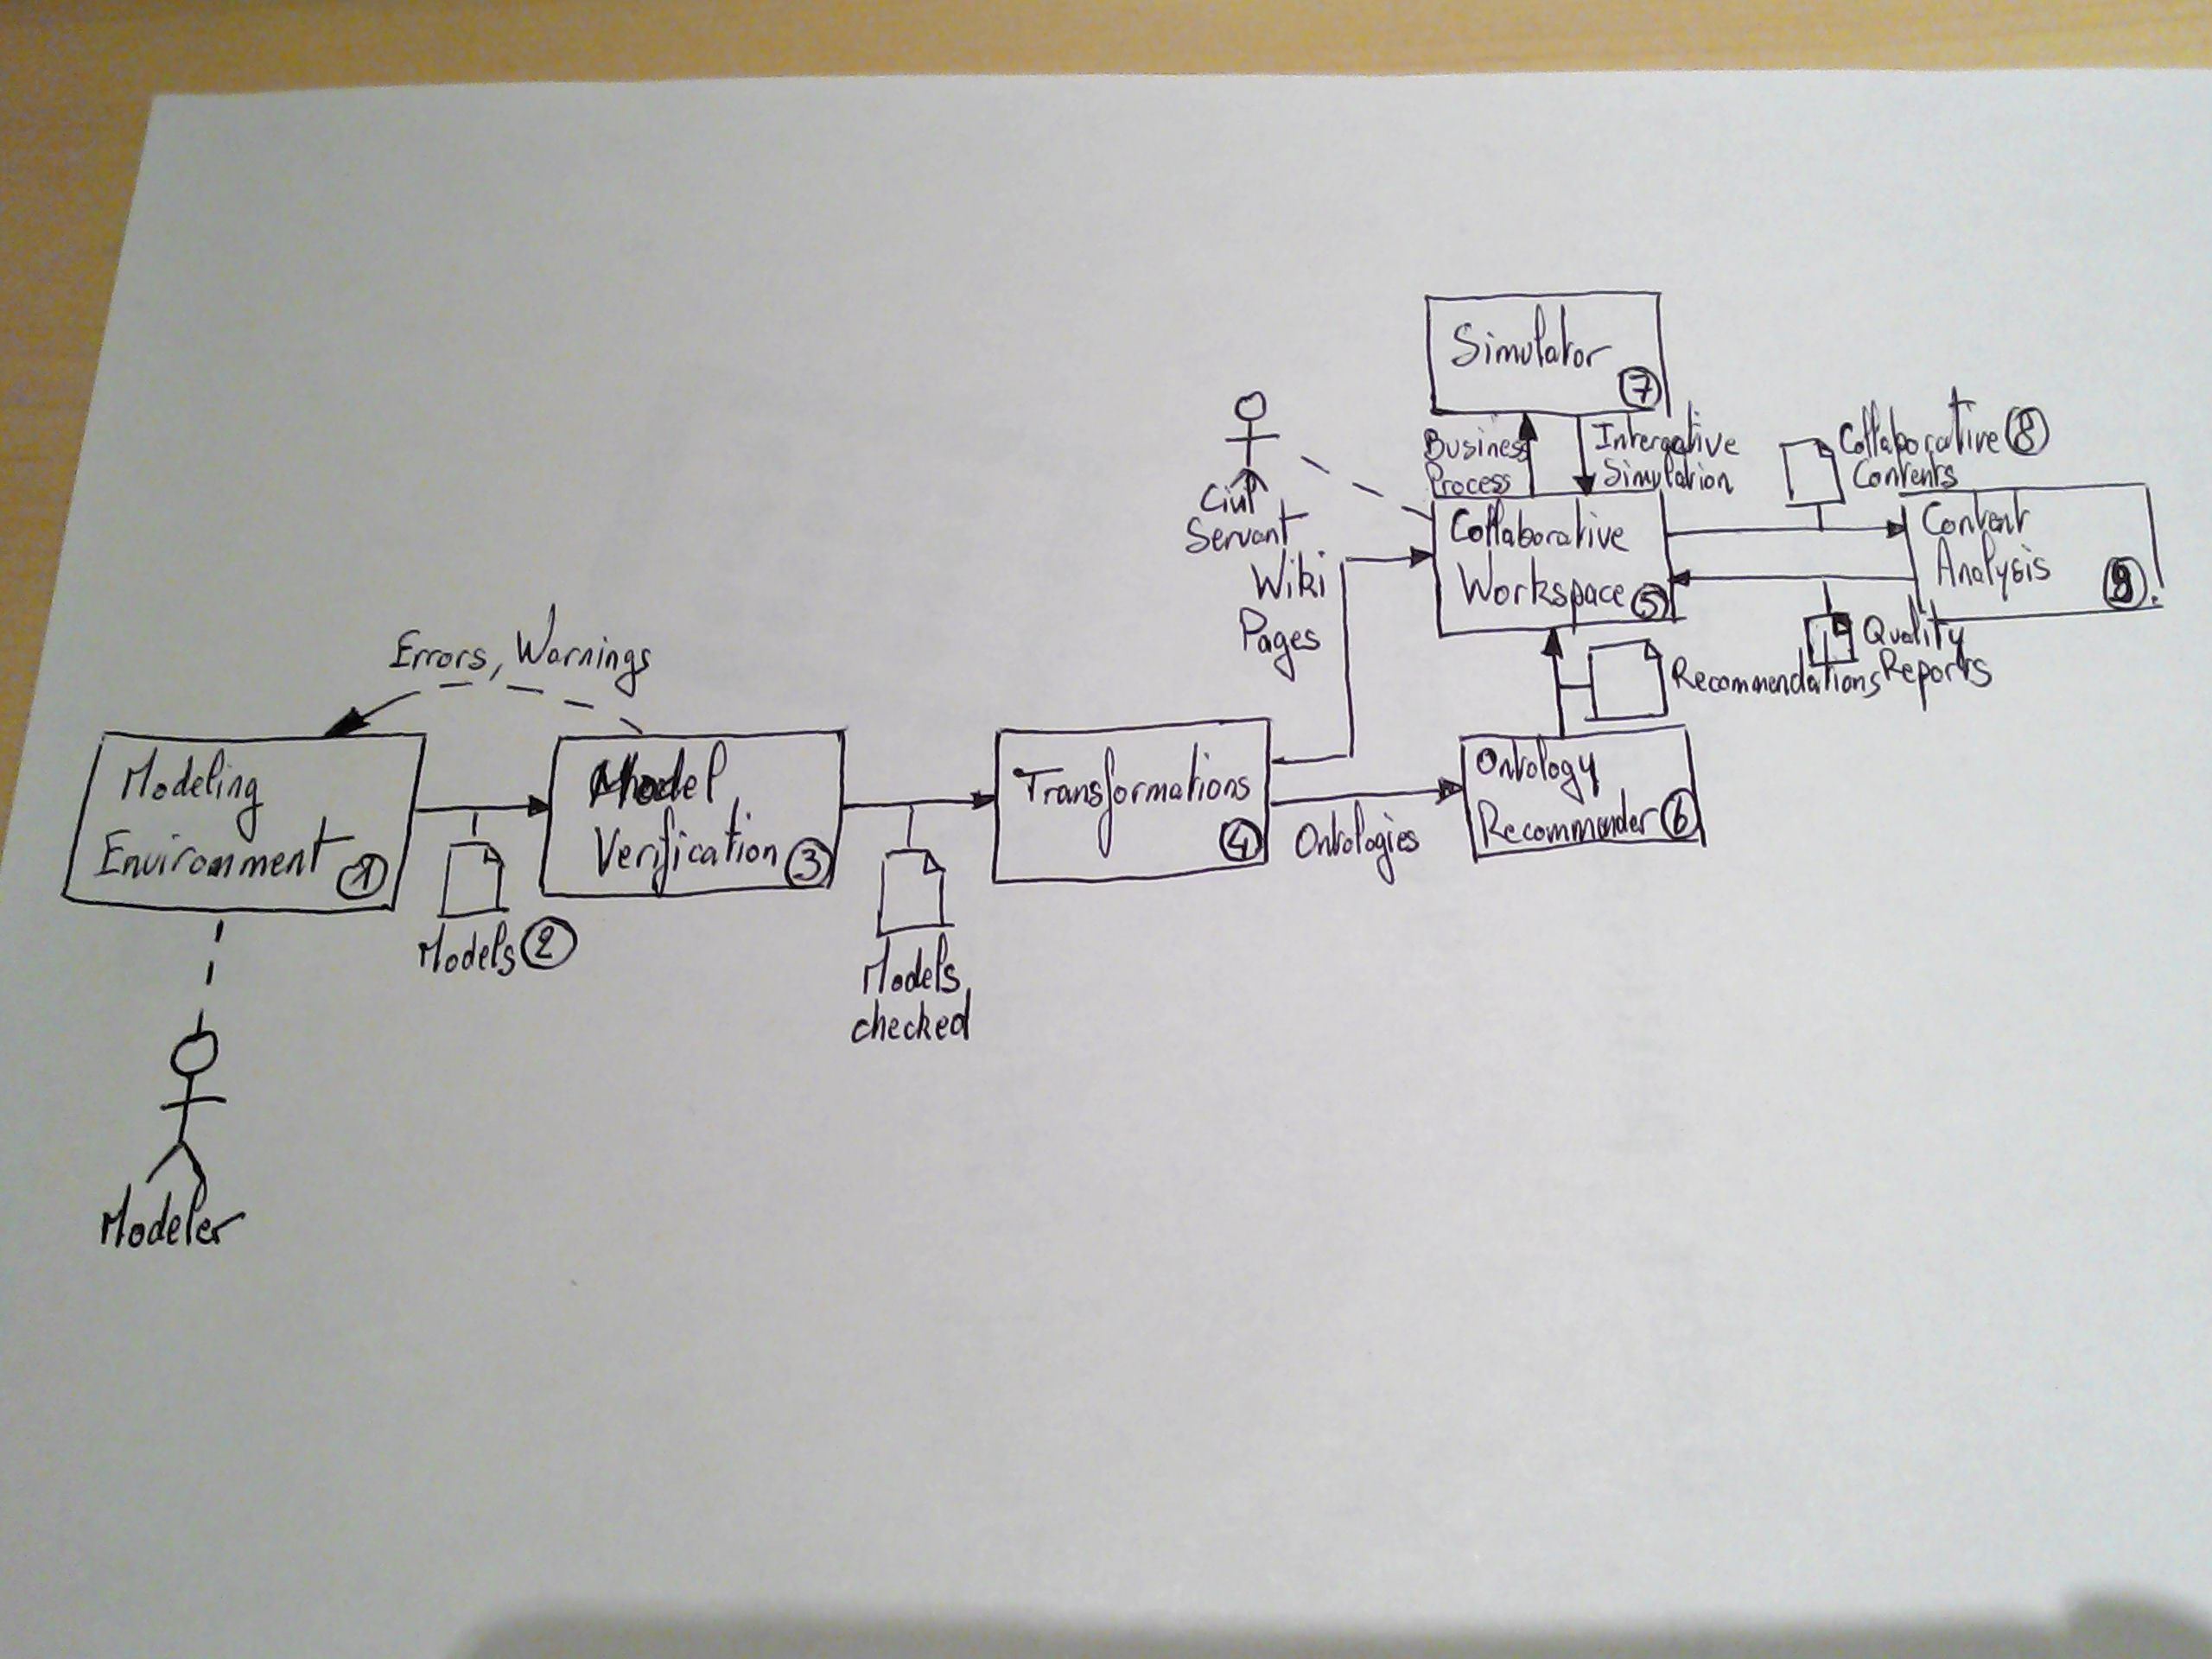
\includegraphics[width=.6\paperwidth,keepaspectratio]{figures/learnpad-flow.jpg}
	\caption{Flow view of the \learnpad platform\newline
	TODO: draw a line between transformation and Simulator to transfer Business Process then remove the one between CW and SIM\newline
	TODO: Change name of Simulator to Simulation Environment\newline
	TODO: Remove the number (2) and update other numbers accordingly\newline
	TODO: Remove the number (8) and update other numbers accordingly}
	\label{fig:flow-view}
\end{figure}

\subsection{Modeling Environment}
\label{sec:modeling-environment}

\paragraph{Technology}
Adoxx, MagicDraw

\paragraph{Description}
In the Modeling Environment, the
Modeler is describing and documenting the models.  Any modeling tool could be
plugged on the \learnpad platform as long as its providing the correct output
format.

The output format contains a few things:
\begin{itemize}
	\item A set of models which are woven together
	\item Clickable images of the models (images and maps)
	\item Business Process models as one BPMN (standard format) file
\end{itemize}

\subsection{Model Verification}
\label{sec:model-verification}

\paragraph{Technology}
PetriNET

\paragraph{Description}
Before importing the models, the \learnpad platform will run a list of
verifications on the models.  These are formal verifications to avoid
importation of models that are not executable or that contains activities that
are not reachable (these are only 2 examples).

\subsection{Transformations}
\label{sec:transformations}

\paragraph{Technology}
EMF, ATL, Acceleo, XSL-T

\paragraph{Description}
Once the model has been validated, it can be imported into the \learnpad
platform.  3 components will need these models for different purposes.

First of all, the Collaborative Workspace will display these models into a wiki
for the Civil Servants.  These transformations are done using Modeling
Transformations tools like EMF (to represent models), ATL (to convert models)
and Acceleo (to serialize EMF representations of models).

On the second hand, the Ontology Recommender has to build an ontology of the
models in order to propose recommendations.  The transformations technology used
here is XML-specific: XSL-Transformations.

Finally, the Simulator will simulate Business Process.  It's using the Activiti
Engine which is able to run simulation on Business Process serialized as BPMN
standard format.

\subsection{Collaborative Workspace}
\label{sec:collaborative-workspace}

\paragraph{Technology}
Wiki

\paragraph{Description}
The Collaborative Workspace is the User Interface entry point for Civil
Servants.  It's in the Collaborative Workspace they will consult, browse, learn
about new or existing processes.

Civil Servants are able to collaborate into this workspace by providing
additionnal documentation, help to fix inconsistent, incomplete or wrong models

\subsection{Ontology Recommender}
\label{sec:ontology-recommender}

\paragraph{Technology}
ArchiMate, ArchiMEO, RDF

\paragraph{Description}
The Ontology Recommender will create an ontology based on the models that are
pushed to him.  This ontology will produce different kind of recommendations to
the Civil Servant as they browse the wiki and use the simulation (see
Section~\ref{sec:simulator}:
\begin{itemize}
	\item \emph{Experts} they could talk to to get more details on the activity
	\item \emph{Similar Cases} which are similar processes to the one currently
		consulted or simulated
	\item \emph{Learning Materials} which are related
		multimedias that can help to understand the activity
\end{itemize}

\subsection{Simulator}
\label{sec:simulator}

\paragraph{Technology}
Activiti, BPMN

\paragraph{Description}
On the Simulator, Civil Servants will be able to interactively simulate a
process, playing each activity of it and validate each step.  It's a learning
tool so the Simulator will give feedback about the expected values.  Multiple
Civil Servants may interact on a common simulation too.  In any case,
gamification mechanisms will keep this exercise motivating for Civil Servants.

\subsection{Content Analysis}
\label{sec:content-analysis}

\paragraph{Technology}
Gate

\paragraph{Description}
In the Collaborative Workspace, the Civil Servants will be able to co-edit new
documents that will complete the processes' documentation.  These documents will
be beneficial for every other Civil Servant.  Therefore, Content Analysis is in
charge of keeping a minimum level of quality for these documents.  It will run
semantic analysis on the produced documents in order to spot vagueness or
incomplete information in the texts.

\section{Component view}
\label{sec:component-view}
The component view will show which are the real existing components and how they
are connected to each other into the \learnpad platform (see
Figure~\ref{fig:component-view}).

\begin{figure}[!htp]
	\centering
	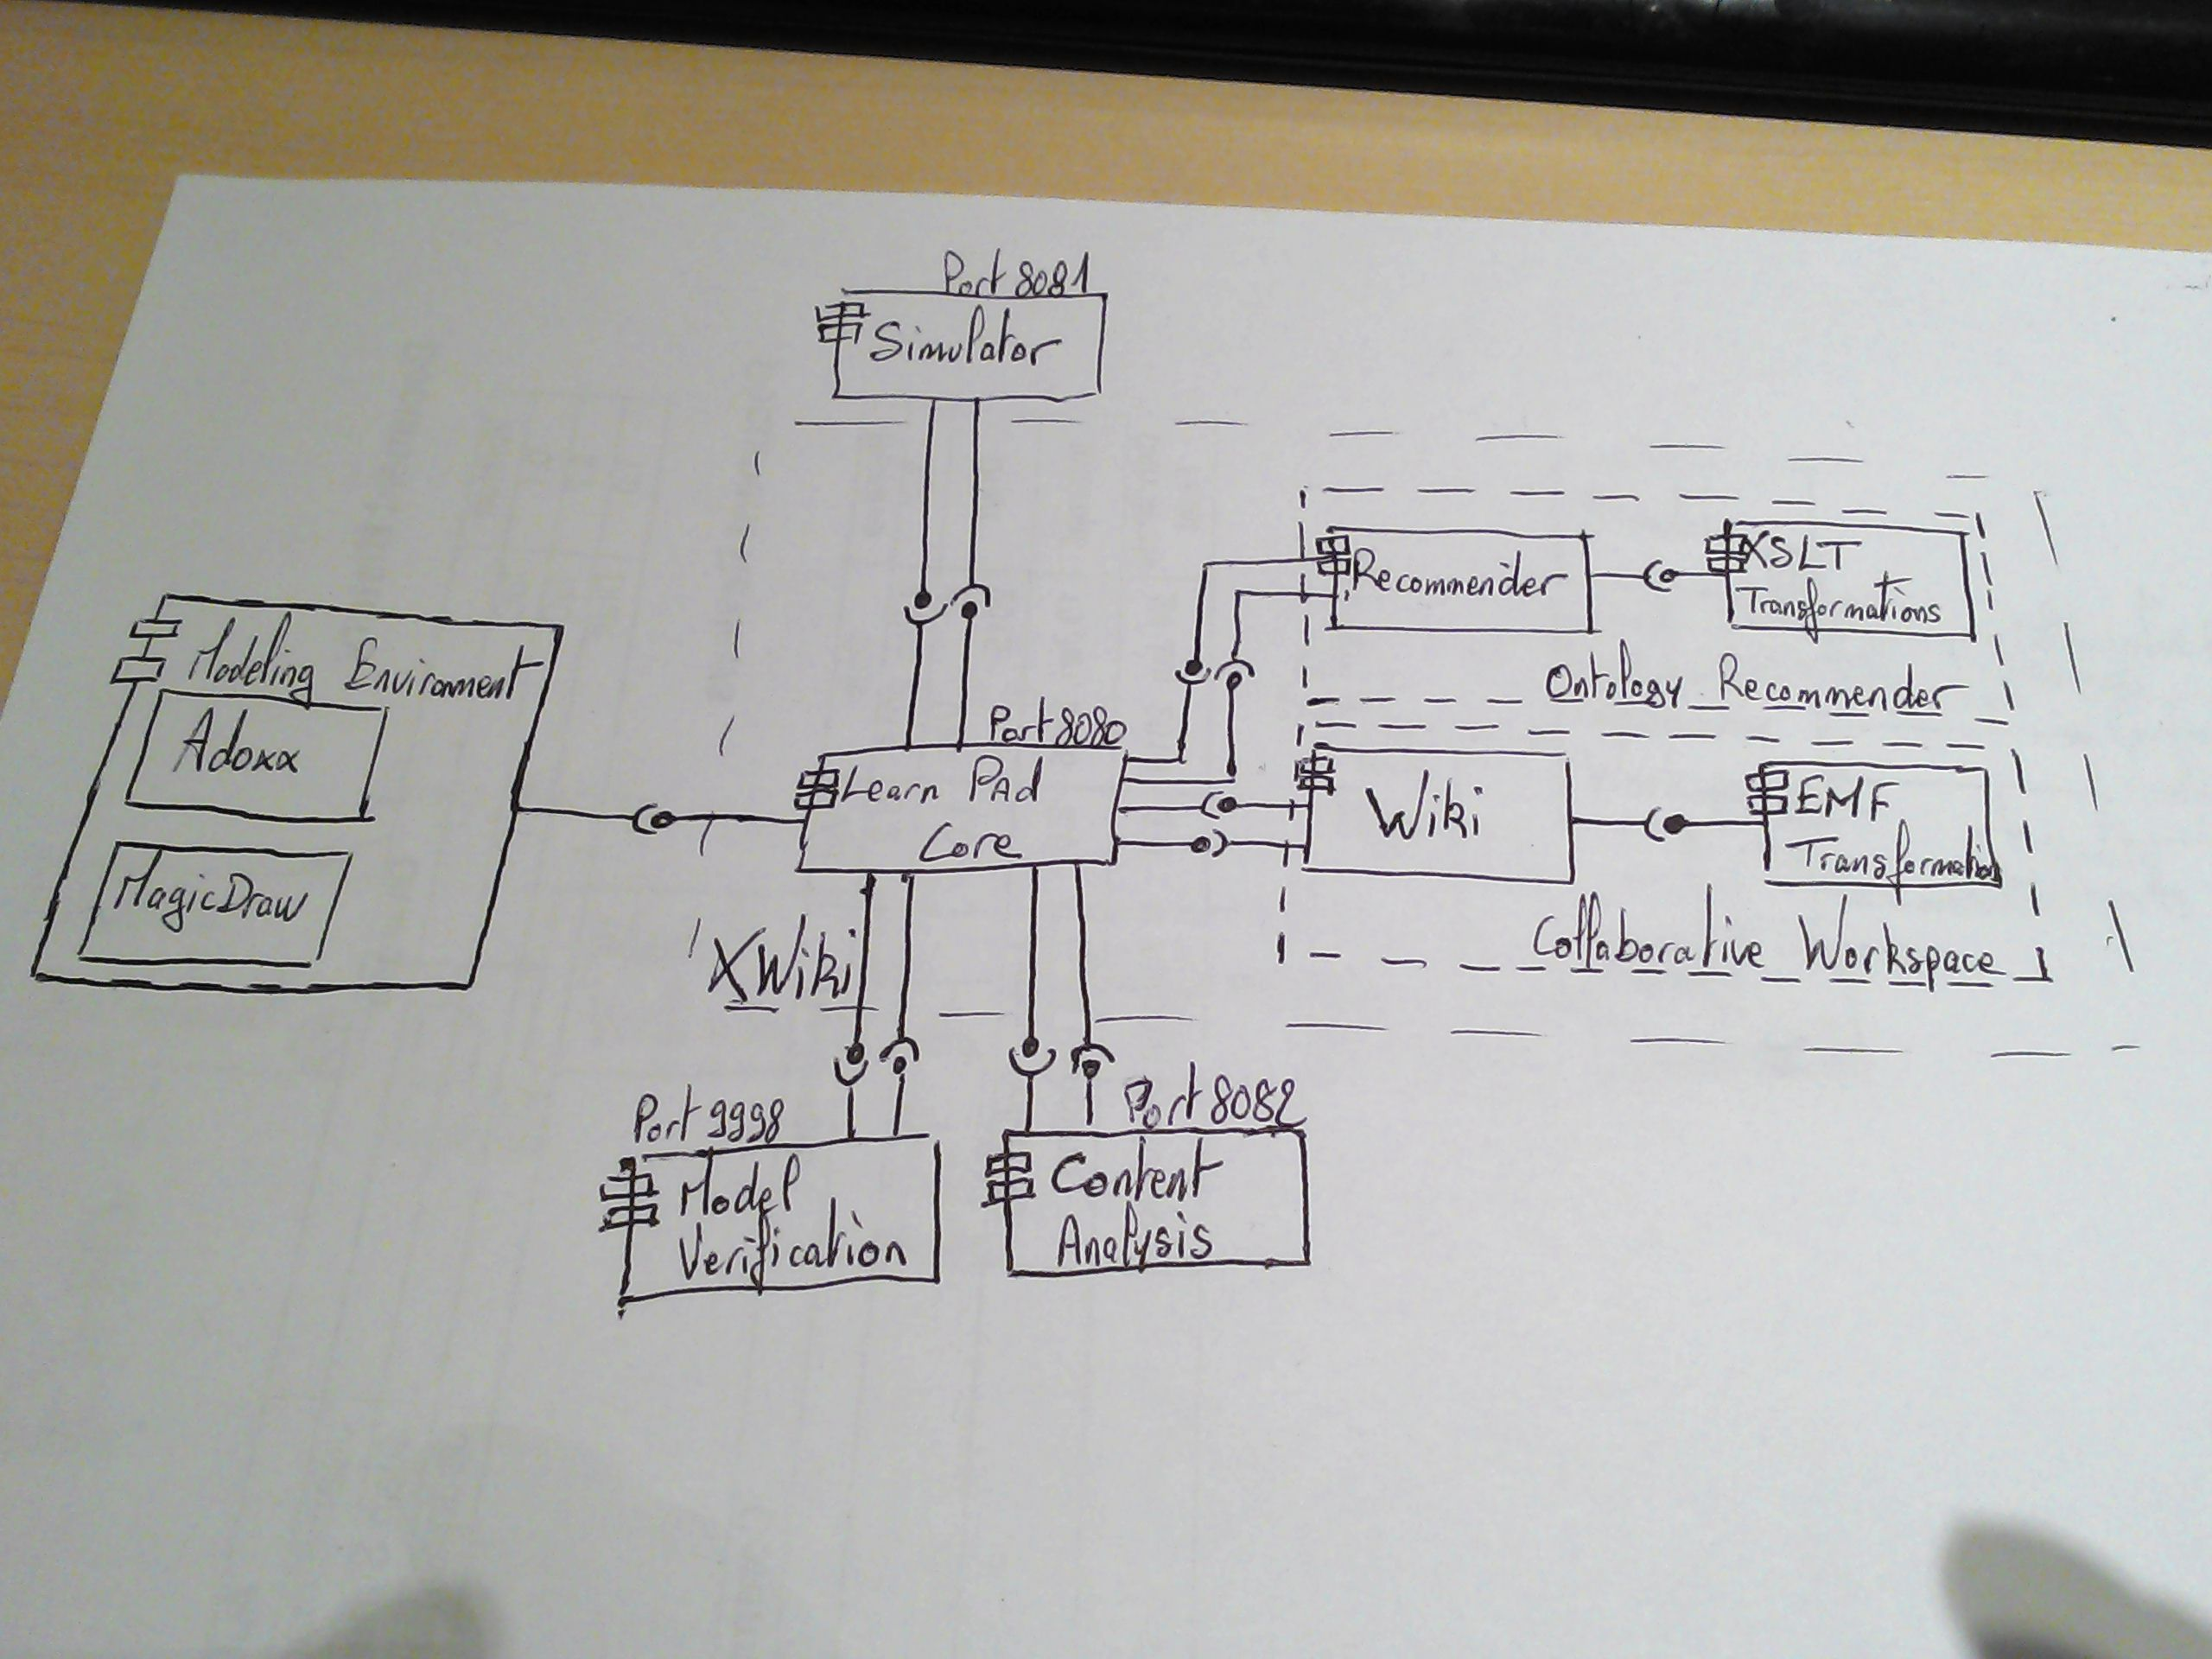
\includegraphics[width=.6\paperwidth,keepaspectratio]{figures/learnpad-architecture.jpg}
	\caption{Component view of the \learnpad platform}
	\label{fig:component-view}
\end{figure}

\subsection{Learn PAd Core}
\learnpad platform has been designed as modular as possible.  Everything is
plugged onto this \learnpad Core.  In order to be independent as much as
possible from the technologies used in each component, each component is
communicating with the \learnpad Core with REST APIs.

This component is developed inside the XWiki software.  This means that storage
is shared with all components that are part of XWiki.  However, it communicates
with all the components with REST which make it a replaceable component.

\subsection{Modeling Environment}
This component is not part of \learnpad platform.  \learnpad platform is a
server providing a list of features and services: it's always on.  However, the
Modeling Environment could be desktop application that is launched, used, then
stopped.  It a necessary component to the \learnpad flow but it's not always on.
That's the reason why its talking to \learnpad Core Platform but never the other
way around.

The format they will push toward the \learnpad platform is a ZIP archive, called \verb+lpzip+ which contains:
\begin{itemize}
	\item Set of models [format:XML/Adoxx or XML/MagicDraw]
	\item Images [format: BMP, JPG, PNG, SVG]
	\item Images map [format:HTML-Map]
	\item Business Process models [format:BPMN2.0]
\end{itemize}

\subsection{Collaborative Workspace}
The Collaborative Workspace is divided into 2 main components.  Since the
\learnpad Core is not doing any transformation on the files (\learnpad Core is
more like a router), the Collaborative Workspace is getting raw files.
Therefore, the Wiki component is getting raw models from the \learnpad Core,
then use a EMF Transformation component to transform models into wiki pages,
before importing them.

\subsubsection{Wiki}
The Wiki component is the most important part of the Collaborative Workspace.
It's the Graphical User Interface for Civil Servants where models will be
displayed.  It contains modeling data, stored with a generic format, and an
application capable of displaying these datas.

Wiki component will get models, ask for transformation, and import the resulting
wiki pages from the transformation.

\subsubsection{EMF Transformation}
This transformation module is using EMF technologies to operate transformations
on models.  Each meta-model is represented as an Ecore module (Adoxx, MagicDraw,
XWiki).  Then, a transformation language, ATL, transform them from an Ecore A
(Adoxx or MagicDraw) to an Ecore B (XWiki).  Finally, Acceleo is serializing the
Ecore to wiki pages which are returned to the Wiki.

\subsection{Ontology Recommender}
For the same reasons than the Collaborative Workspace, the Ontology Recommender
is getting raw files from \learnpad Core.  Therefore, the main component
Recommender is getting these files, sending them to the XSL-T Transformations
component which return back ontologies of the models.

\subsubsection{Recommender}
The Recommender component is using an ontology to organize the information of
the models.  The ontology is expressed as a RDF format.  This component will be
able to make recommendations to a Civil Servants as he browse a model or play a
simulation.  Contextual information will be used to get the best possible
recommendations, for example:
\begin{itemize}
	\item Who is the current Civil Servant?
	\item What is the Civil Servant is currently looking at?
	\item In case of simulation, what are the data already filled by the Civil
		Servant?
\end{itemize}

\subsubsection{XSL-T Transformations}
This component is transforming models into ontologies.  The technology used is
XML specific, and very efficient as parsing XML files to transform them into
other serialization, RDF ontologies in this case.

\subsection{Simulator}
The Simulator is using Activiti Engine to play simulations of Business
Processes.  Activiti Engine is using BPMN standard format which are already
stored in the \learnpad Core.

The Simulator component is also generating Graphical User Interface for the
Civil Servant.  However, these GUI are embedded inside the Wiki for 2 reasons:
\begin{itemize}
	\item Reduce the number of entry points for the Civil Servants
	\item Display recommendations during the simulation (UI for recommendation
		already exists in the Wiki)
\end{itemize}

\subsection{Model Verification}
The Model Verification is in charge of verifying consistency of models.  It 
runs multiple tests on models in order to identify different kind of errors.  The
Modeling Environment is able to ask \learnpad Core for these errors in order to
show them to the modelers.

\subsection{Content Analysis}
The Content Analysis runs semantic analysis on free text collaboratively created
by Civil Servants in the Wiki.  It returns annotations on the text with the
following information:
\begin{itemize}
	\item Start and End of the piece of concerned text
	\item The type of error (among a list of categories)
\end{itemize}

The annotations are then displayed in the Wiki, providing a workflow to a Civil
Servant for a throrough review of each of these.

\chapter{About partners}
\label{ch:partners}

\section{Consiglio Nazionale delle Ricerche}
Leading partner of the \learnpad project, CNR is an Italian Public Research
Institute.  It's the expert in automatic semantic analysis (for the Content
Analysis component).

\begin{figure}[!htp]
	\centering
	
\includegraphics[width=6em,keepaspectratio]{figures/cnr.png}\par
	\url{http://www.cnr.it}
\end{figure}

\section{BOC Asset Management GmbH}
Based in Austria, it's a leading company in Modeling.  It's providing the
software Adoxx for the Modeling Environment component.

\begin{figure}[!htp]
	\centering
	
\includegraphics[width=6em,keepaspectratio]{figures/boc-group.png}\par
	\url{http://www.boc-group.com}
\end{figure}

\section{Linagora Grand Sud Ouest SA}
Linagora is an open-source company, based in France.  It's providing
technologies and knowledge about execution and simulation of Business Processes.

\begin{figure}[!htp]
	\centering
	
\includegraphics[width=6em,keepaspectratio]{figures/linagora.png}\par
	\url{http://www.linagora.com}
\end{figure}

\section{No Magic Europe UAB}
Based in Lithuania, it's a leading company in Modeling.  It's providing the
software MagicDraw for the Modeling Environment component.

\begin{figure}[!htp]
	\centering
	
\includegraphics[width=6em,keepaspectratio]{figures/nme.png}\par
	\url{http://www.nomagic.com}
\end{figure}

\section{Regione Marche}
Italian Public Administration of the Marche region, it's providing expertise on
processes in Public Administration.

\begin{figure}[!htp]
	\centering
	
\includegraphics[width=6em,keepaspectratio]{figures/marche.jpg}\par
	\url{http://www.regione.marche.it}
\end{figure}

\section{Fachhochschule Nordwestschweiz}
Swiss University with expertise on ontologies.  It's working on the
recommendation engine.

\begin{figure}[!htp]
	\centering
	
\includegraphics[width=6em,keepaspectratio]{figures/fhnw.jpg}\par
	\url{http://www.fhnw.ch}
\end{figure}

\section{Università degli Studi di Camerino}
This Italian University is having expertise in Business Process.  It's working
on formal verification of processes.

\begin{figure}[!htp]
	\centering
	
\includegraphics[width=6em,keepaspectratio]{figures/unicam.png}\par
	\url{http://www.unicam.it}
\end{figure}

\section{Università degli Studi dell'Aquila}
This Italian University is having expertise in models (transformations,
comparisons, historic, etc.) and in the related technologies (EMF, ATL, Acceleo,
EMFCompare, etc.).

\begin{figure}[!htp]
	\centering
	
\includegraphics[width=6em,keepaspectratio]{figures/univaq.png}\par
	\url{http://www.univaq.it}
\end{figure}

\section{XWiki SAS}
French open-source company, which is developing XWiki software.  It's providing
XWiki as the base of the \learnpad platform and expertise about collaboration
and knowledge management.

\begin{figure}[!htp]
	\centering
	
\includegraphics[width=6em,keepaspectratio]{figures/xwiki.png}\par
	\url{http://www.xwiki.com}
\end{figure}

% ---------------------------------- Start with annexes here!
% ----------------------------------

% \annex{}

% ---------------------------------- Start EndNotes here!  
% ---------------------------------- 

% Plese use this command if and only if your text includes endnotes.
% Otherwise, comment it.

% \theendnotes

% ---------------------------------- Bibliography starts here
% ----------------------------------

% \bibliographystyle{plain}
% \bibliography{biblio}

\end{document}
